% !TeX root = paper.tex
%  LaTeX support: latex@mdpi.com 
%  For support, please attach all files needed for compiling as well as the log file, and specify your operating system, LaTeX version, and LaTeX editor.

%=================================================================
\documentclass[journal,article,submit,pdftex,moreauthors]{Definitions/mdpi} 
\usepackage[utf8]{inputenc}
\usepackage{tikz}
\usetikzlibrary{positioning, arrows.meta, shapes.geometric, calc, fit, backgrounds}
%\documentclass[preprints,article,submit,pdftex,moreauthors]{Definitions/mdpi} 
% For posting an early version of this manuscript as a preprint, you may use "preprints" as the journal. Changing "submit" to "accept" before posting will remove line numbers.

% Below journals will use APA reference format:
% admsci, aieduc, behavsci, businesses, econometrics, economies, education, ejihpe, famsci, games, humans, ijcs, ijfs, jintelligence, journalmedia, jrfm, jsam, languages, peacestud, psycholint, publications, tourismhosp, youth

% Below journals will use Chicago reference format:
% arts, genealogy, histories, humanities, laws, literature, religions, risks, socsci

%--------------------
% Class Options:
%--------------------
%----------
% journal
%----------
% Choose between the following MDPI journals:
% accountaudit, acoustics, actuators, addictions, adhesives, admsci, adolescents, aerobiology, aerospace, agriculture, agriengineering, agrochemicals, agronomy, ai, aichem, aieduc, aieng, aimater, aimed, aipa, air, aisens, algorithms, allergies, alloys, amh, analog, analytica, analytics, anatomia, anesthres, animals, antibiotics, antibodies, antioxidants, applbiosci, appliedchem, appliedmath, appliedphys, applmech, applmicrobiol, applnano, applsci, aquacj, architecture, arm, arthropoda, arts, asc, asi, astronautics, astronomy, atmosphere, atoms, audiolres, automation, axioms, bacteria, batteries, bdcc, behavsci, beverages, biochem, bioengineering, biologics, biology, biomass, biomechanics, biomed, biomedicines, biomedinformatics, biomimetics, biomolecules, biophysica, bioresourbioprod, biosensors, biosphere, biotech, birds, blockchains, bloods, blsf, brainsci, breath, buildings, businesses, cancers, carbon, cardio, cardiogenetics, cardiovascmed, catalysts, cells, ceramics, challenges, chemengineering, chemistry, chemosensors, chemproc, children, chips, cimb, civileng, cleantechnol, climate, clinbioenerg, clinpract, clockssleep, cmd, cmtr, coasts, coatings, colloids, colorants, commodities, complexities, complications, compounds, computation, computers, condensedmatter, conservation, constrmater, cosmetics, covid, crops, cryo, cryptography, crystals, csmf, ctn, culture, curroncol, cyber, dairy, data, ddc, dentistry, dermato, dermatopathology, designs, devices, dhi, diabetology, diagnostics, dietetics, digital, disabilities, diseases, diversity, dna, drones, dynamics, earth, ebj, ecm, ecologies, econometrics, economies, edm, education, eesp, ejihpe, electricity, electrochem, electronicmat, electronics, encyclopedia, endocrines, energies, eng, engproc, entomology, entropy, environments, environremediat, epidemiologia, epigenomes, esa, est, famsci, fermentation, fibers, fintech, fire, fishes, fluids, foods, forecasting, forensicsci, forests, fossstud, foundations, fractalfract, fuels, future, futureinternet, futurepharmacol, futurephys, futuretransp, galaxies, games, gases, gastroent, gastrointestdisord, gastronomy, gels, genealogy, genes, geographies, geohazards, geomatics, geometry, geosciences, geotechnics, geriatrics, germs, glacies, grasses, green, greenhealth, gucdd, hardware, hazardousmatters, healthcare, hearts, hemato, hematolrep, hep, heritage, higheredu, highthroughput, histories, horticulturae, hospitals, humanities, humans, hydrobiology, hydrogen, hydrology, hydropower, hygiene, idr, iic, ijcs, ijem, ijerph, ijfs, ijgi, ijmd, ijms, ijns, ijom, ijpb, ijt, ijtm, ijtpp, ime, immuno, informatics, information, infrastructures, inorganics, insects, instruments, inventions, iot, j, jaestheticmed, jal, jcdd, jcm, jcp, jcrm, jcs, jcto, jdad, jdb, jdream, jemr, jeta, jfb, jfmk, jgbg, jgg, jimaging, jintelligence, jlpea, jmahp, jmmp, jmms, jmp, jmse, jne, jnt, jof, joi, joitmc, joma, jop, joptm, jor, journalmedia, jox, jpbi, jphytomed, jpm, jrfm, jsam, jsan, jtaer, jvd, jzbg, kidneydial, kinasesphosphatases, knowledge, labmed, laboratories, lae, land, languages, laws, life, lights, limnolrev, lipidology, liquids, literature, livers, logics, logistics, lubricants, lymphatics, machines, macromol, magnetism, magnetochemistry, make, marinedrugs, materials, materproc, mathematics, mca, measurements, medicina, medicines, medsci, membranes, merits, metabolites, metals, meteorology, methane, metrics, metrology, micro, microarrays, microbiolres, microelectronics, micromachines, microorganisms, microplastics, microwave, minerals, mining, mmphys, modelling, molbank, molecules, mps, msf, mti, multimedia, muscles, nanoenergyadv, nanomanufacturing, nanomaterials, ncrna, ndt, network, neuroglia, neuroimaging, neurolint, neurosci, nitrogen, notspecified, nursrep, nutraceuticals, nutrients, obesities, occuphealth, oceans, ohbm, onco, optics, oral, organics, organoids, osteology, oxygen, pandemics, parasites, parasitologia, particles, pathogens, pathophysiology, peacestud, pediatrrep, pets, pharmaceuticals, pharmaceutics, pharmacoepidemiology, pharmacy, philosophies, photochem, photonics, phycology, physchem, physics, physiologia, plants, plasma, platforms, pollutants, polymers, polysaccharides, populations, poultry, powders, precipitation, precisoncol, preprints, proceedings, processes, prosthesis, proteomes, psf, psychiatryint, psychoactives, psycholint, publications, purification, quantumrep, quaternary, qubs, radiation, rdt, reactions, realestate, receptors, recycling, regeneration, religions, remotesensing, reports, reprodmed, resources, rheumato, risks, rjpm, robotics, rsee, ruminants, safety, sci, scipharm, sclerosis, seeds, sensors, separations, sexes, shi, signals, sinusitis, siuj, skins, smartcities, sna, societies, socsci, software, soilsystems, solar, solids, spectroscj, sports, standards, stats, std, stratsediment, stresses, surfaces, surgeries, suschem, sustainability, symmetry, synbio, systems, tae, targets, taxonomy, technologies, telecom, test, textiles, thalassrep, therapeutics, thermo, timespace, tomography, tourismhosp, toxics, toxins, tph, transplantology, transportation, traumacare, traumas, tri, tropicalmed, universe, urbansci, uro, vaccines, vehicles, venereology, vetsci, vibration, virtualworlds, viruses, vision, waste, water, welding, wem, wevj, wild, wind, women, world, youth, zoonoticdis

%---------
% article
%---------
% The default type of manuscript is "article", but can be replaced by: 
% abstract, addendum, article, benchmark, book, bookreview, briefcommunication, briefreport, casereport, changes, clinicopathologicalchallenge, comment, commentary, communication, conceptpaper, conferenceproceedings, correction, conferencereport, creative, datadescriptor, discussion, entry, expressionofconcern, extendedabstract, editorial, essay, erratum, fieldguide, hypothesis, interestingimages, letter, meetingreport, monograph, newbookreceived, obituary, opinion, proceedingpaper, projectreport, reply, retraction, review, perspective, protocol, shortnote, studyprotocol, supfile, systematicreview, technicalnote, viewpoint, guidelines, registeredreport, tutorial,  giantsinurology, urologyaroundtheworld
% supfile = supplementary materials

%----------
% submit
%----------
% The class option "submit" will be changed to "accept" by the Editorial Office when the paper is accepted. This will only make changes to the frontpage (e.g., the logo of the journal will get visible), the headings, and the copyright information. Also, line numbering will be removed. Journal info and pagination for accepted papers will also be assigned by the Editorial Office.

%------------------
% moreauthors
%------------------
% If there is only one author the class option oneauthor should be used. Otherwise use the class option moreauthors.

%---------
% pdftex
%---------
% The option pdftex is for use with pdfLaTeX. Remove "pdftex" for (1) compiling with LaTeX & dvi2pdf (if eps figures are used) or for (2) compiling with XeLaTeX.

%=================================================================
% MDPI internal commands - do not modify
\firstpage{1} 
\makeatletter 
\setcounter{page}{\@firstpage} 
\makeatother
\pubvolume{1}
\issuenum{1}
\articlenumber{0}
\pubyear{2026}
\copyrightyear{2025}
%\externaleditor{Firstname Lastname} % More than 1 editor, please add `` and '' before the last editor name
\datereceived{ } 
\daterevised{ } % Comment out if no revised date
\dateaccepted{ } 
\datepublished{ } 
%\datecorrected{} % For corrected papers: "Corrected: XXX" date in the original paper.
%\dateretracted{} % For retracted papers: "Retracted: XXX" date in the original paper.
%\doinum{} % Used for some special journals, like molbank
%\pdfoutput=1 % Uncommented for upload to arXiv.org
%\CorrStatement{yes}  % For updates
%\longauthorlist{yes} % For many authors that exceed the left citation part
%\IsAssociation{yes} % For association journals

%=================================================================
% Add packages and commands here. The following packages are loaded in our class file: fontenc, inputenc, calc, indentfirst, fancyhdr, graphicx, epstopdf, lastpage, ifthen, float, amsmath, amssymb, lineno, setspace, enumitem, mathpazo, booktabs, titlesec, etoolbox, tabto, xcolor, colortbl, soul, multirow, microtype, tikz, totcount, changepage, attrib, upgreek, array, tabularx, pbox, ragged2e, tocloft, marginnote, marginfix, enotez, amsthm, natbib, hyperref, cleveref, scrextend, url, geometry, newfloat, caption, draftwatermark, seqsplit
% cleveref: load \crefname definitions after \begin{document}

%=================================================================
% Please use the following mathematics environments: Theorem, Lemma, Corollary, Proposition, Characterization, Property, Problem, Example, ExamplesandDefinitions, Hypothesis, Remark, Definition, Notation, Assumption
%% For proofs, please use the proof environment (the amsthm package is loaded by the MDPI class).

%=================================================================
% Full title of the paper (Capitalized)
\Title{Interpretability in Deep Knowledge Tracing - A Theory-Guided Approach}

% Author Orchid ID: enter ID or remove command
\newcommand{\orcidauthorA}{0009-0004-3499-6106} % Add \orcidA{} behind the author's name
\newcommand{\orcidauthorB}{0000-0002-9281-4209} % Add \orcidB{} behind the author's name

% Authors, for the paper (add full first names)
\Author{Concha Labra $^{1}$\orcidA{}, Olga C. Santos $^{2,*}$\orcidB{}}

%\longauthorlist{yes}

% MDPI internal command: Authors, for metadata in PDF
\AuthorNames{Concha Labra, Olga C. Santos}

%\longauthorlist{yes}

% Affiliations / Addresses (Add [1] after \address if there is only one affiliation.)
\address{%
$^{1}$ \quad Department of Artificial Intelligence, Computer Science School, UNED, 28040 Madrid, Spain; clabra@dia.uned.es\\
$^{2}$ \quad PhyUM Research Center, Department of Artificial Intelligence, Computer Science School, UNED, 28040 Madrid, Spain; ocsantos@dia.uned.es}

% Contact information of the corresponding author
\corres{Author to whom correspondence should be addressed.}

% Current address and/or shared authorship
%\firstnote{Current address: Affiliation.}  
% Current address should not be the same as any items in the Affiliation section.

%\secondnote{These authors contributed equally to this work.}
% The commands \thirdnote{} till \eighthnote{} are available for further notes.

%\simplesumm{} % Simple summary

%\conference{} % An extended version of a conference paper

% Abstract (Do not insert blank lines, i.e. \\) 
\abstract{This study introduces iDKT, an interpretable-by-design Transformer model that utilizes \textit{Representational Grounding} to align deep latent representations with educational constructs, leveraging the high accuracy of deep knowledge tracing models while addressing their inherent lack of interpretability. We introduce a formal validation framework to verify the alignment of iDKT's internal representations and, using Bayesian Knowledge Tracing (BKT) as a reference, evaluate the model across multiple educational datasets. Results demonstrate that iDKT maintains state-of-the-art predictive performance while yielding additional interpretable insights at a significantly higher granularity than those provided by the reference model. Specifically, iDKT identifies student-level initial knowledge and learning velocities, providing mastery estimates that are more sensitive to the nuances of individual behavioral patterns than those produced by standard BKT. These individualized insights enable precise diagnostic placement and dynamic pacing, allowing adaptive learning environments to tailor instruction to each student's unique learning profile with enhanced precision. This work offers both a robust methodology for evaluating the interpretability of Transformer-based models and a practical tool for improving educational effectiveness through data-driven personalization.} 

% Keywords
\keyword{deep knowledge tracing; transformer; interpretability; Bayesian Knowledge Tracing; educational data analysis; personalized learning} 

% The fields PACS, MSC, and JEL may be left empty or commented out if not applicable
%\PACS{J0101}
%\MSC{}
%\JEL{}

%%%%%%%%%%%%%%%%%%%%%%%%%%%%%%%%%%%%%%%%%%
% Only for the journal Diversity
%\LSID{\url{http://}}

%%%%%%%%%%%%%%%%%%%%%%%%%%%%%%%%%%%%%%%%%%
% Only for the journal Applied Sciences
%\featuredapplication{Authors are encouraged to provide a concise description of the specific application or a potential application of the work. This section is not mandatory.}
%%%%%%%%%%%%%%%%%%%%%%%%%%%%%%%%%%%%%%%%%%

%%%%%%%%%%%%%%%%%%%%%%%%%%%%%%%%%%%%%%%%%%
% Only for the journal Data
%\dataset{DOI number or link to the deposited data set if the data set is published separately. If the data set shall be published as a supplement to this paper, this field will be filled by the journal editors. In this case, please submit the data set as a supplement.}
%\datasetlicense{License under which the data set is made available (CC0, CC-BY, CC-BY-SA, CC-BY-NC, etc.)}

%%%%%%%%%%%%%%%%%%%%%%%%%%%%%%%%%%%%%%%%%%
% Only for the journal BioTech, Fishes, Neuroimaging and Toxins
%\keycontribution{The breakthroughs or highlights of the manuscript. Authors can write one or two sentences to describe the most important part of the paper.}

%%%%%%%%%%%%%%%%%%%%%%%%%%%%%%%%%%%%%%%%%%
% Only for the journal Encyclopedia
%\encyclopediadef{For entry manuscripts only: please provide a brief overview of the entry title instead of an abstract.}

%%%%%%%%%%%%%%%%%%%%%%%%%%%%%%%%%%%%%%%%%%
% Different journals have different requirements. Please check the specific journal guidelines in the "Instructions for Authors" on the journal's official website.
%\addhighlights{yes}
%\renewcommand{\addhighlights}{%
%
%\noindent The goal is to increase the discoverability and readability of the article via search engines and other scholars. Highlights should not be a copy of the abstract, but a simple text allowing the reader to quickly and simplified find out what the article is about and what can be cited from it. Each of these parts should be devoted up to 2~bullet points.\vspace{3pt}\\
%\textbf{What are the main findings?}
% \begin{itemize}[labelsep=2.5mm,topsep=-3pt]
% \item First bullet.
% \item Second bullet.
% \end{itemize}\vspace{3pt}
%\textbf{What are the implications of the main findings?}
% \begin{itemize}[labelsep=2.5mm,topsep=-3pt]
% \item First bullet.
% \item Second bullet.
% \end{itemize}
%}

%%%%%%%%%%%%%%%%%%%%%%%%%%%%%%%%%%%%%%%%%%
\begin{document}

%%%%%%%%%%%%%%%%%%%%%%%%%%%%%%%%%%%%%%%%%%


\section{Introduction}

Knowledge Tracing \citep{corbett1994knowledge} is a fundamental task in the fields of Artificial Intelligence in Education, Intelligent Tutoring Systems and Massive Open Online Courses. Its primary objective is to model a student's dynamic knowledge state over time based on their history of interactions with learning materials, enabling systems to predict future performance and provide personalized instruction. As educational environments become increasingly diverse and digital, the ability to accurately track and interpret student mastery has become a critical requirement for scalable, effective education. 

Historically, the field has been dominated by two distinct paradigms. The first, exemplified by Bayesian Knowledge Tracing (BKT) and its variants \citep{twenty_five_years_of_bkt}, relies on probabilistic graphical models that explicitly represent knowledge states. BKT models are intrinsically interpretable, being based on parameters such as initial knowledge, learning rate, or slipping and guessing probabilities that map directly to pedagogical constructs, allowing educators to understand how they work and trust their decisions. However, this interpretability comes at the cost of a simplicity that often limits its predictive power, making them struggle to capture the complex, non-linear dependencies often present in educational datasets. 

The second paradigm emerged with the advent of Deep Knowledge Tracing (DKT) \citep{piech2015deep}, which uses different variants of deep learning techniques from the initial Recurrent Neural Networks to current Transformers \citep{vaswani2017attention} to model student interactions. These models have achieved state-of-the-art predictive performance, significantly outperforming classical approaches by leveraging the high capacity of deep learning models that allows them to learn complex patterns \citep{abdelrahman2023knowledge}. Yet, this predictive power has come at a significant cost: interpretability. Deep learning models are notoriously opaque "black boxes," where the learned representations are distributed across high-dimensional latent spaces that bear no direct correspondence to constructs with a clear semantic meaning. This lack of transparency creates a trust gap for practitioners, who cannot easily discern why a model predicts a student has failed or succeeded, nor can derive actionable pedagogical insights from the model's internal state \citep{bai2024survey}. 

Current efforts to bridge this gap typically rely on post-hoc explainability methods, such as weights visualization or perturbation analysis \citep{fantozzi2024explainability, di2025ante}. While valuable for debugging, these techniques often provide only a superficial view of the model's decision-making process and do not guarantee that the learned representations align with meaningful constructs. Moreover, their application and interpretation require technical deep learning expertise, limiting their accessibility to practitioners without this specialized knowledge. 

To address these limitations, we propose a shift towards interpretability-by-design, inspired by the emerging paradigm of Theory-Guided Data Science (TGDS) \citep{karpatne2017theory}. In TGDS, maintaining consistency with theoretical postulates is an architectural constraint rather than an afterthought. By integrating extensive domain knowledge, TGDS-based models can be constrained to learn representations that are both theoretically plausible and highly predictive. While this approach has been applied mostly to science—and specifically to physics \citep{willard2022integrating}—we adapt it here to the educational domain.

Standard TGDS implementations typically rely on auxiliary loss functions to incorporate formal knowledge expressed as rules, algebraic constraints, or differential equations \citep{vonrueden2021informed}. We propose a novel approach called \textit{Representational Grounding} that, in contrast, utilizes auxiliary losses operating on projections of the Transformer's embeddings. This mechanism enables the model to learn representations that are consistent with semantically meaningful constructs.

The major contributions of this work are as follows:
\begin{itemize}
    \item Proposal of Representational Grounding, a novel method that overcomes the black-box nature of Transformers by providing interpretability-by-design.
    \item Introduction of a formal validation framework to quantify interpretability via representational alignment, enabling a systematic characterization of the trade-off between reference fidelity and predictive performance.
    \item Application of Representational Grounding to the development of iDKT, a new type of knowledge tracing models that leverage the high accuracy inherent in deep learning while achieving pedagogical interpretability.
    \item Empirical demonstration of iDKT benefits by showing how it captures granular, student-specific insights—such as individualized initial knowledge and learning rates—that are beyond the capabilities of simpler models such as BKT.
\end{itemize}


The remainder of this paper is structured as follows. Section~\ref{sec_related} reviews related work on knowledge tracing, deep learning interpretability, and theory-guided data science. Section~\ref{sec_arch} describes the proposed iDKT architecture and the \textit{Representational Grounding} framework. Sections~\ref{sec_embeddings} and \ref{sec_loss} detail the individualized embedding mechanism and the multi-objective loss system, respectively. Section~\ref{sec_experiment} presents the results of the experimental validation, interpretability results, and the analysis of individualization granularity. Finally, Section~\ref{sec_conclusions} concludes the paper.



%%%%%%%%%%%%%%%%%%%%%%%%%%%%%%%%%%%%%%%%%%
\section{Related Work} \label{sec_related}
\subsection{Deep Knowledge Tracing}
\subsection{Bayesian Knowledge Tracing}
\subsubsection{Parameters of the Standard Model}
\subsubsection{Individualization}
\subsection{Deep Learning Interpretability}
\subsection{Theory-Guided Data Science}
%%%%%%%%%%%%%%%%%%%%%%%%%%%%%%%%%%%%%%%%%%

\section{iDKT Model} \label{sec_arch}

We propose an Interpretable Deep Knowledge Tracing (iDKT) model with a Transformer-based architecture designed to bridge the gap between the high predictive capacity of deep learning and the intrinsic interpretability of simpler models such as Bayesian Knowledge Tracing (BKT). Unlike standard black-box models, iDKT utilizes a novel mechanism called Representational Grounding to anchor its latent representations to the conceptual space of a interpretable model choosen as reference. 

The core architecture of iDKT, as illustrated in Figure~\ref{idkt_arch}, extends the standard Transformer framework \citep{vaswani2017attention} by incorporating specialized components for Representational Grounding, primarily integrated within the embedding layers and the multi-objective loss pipeline.\begin{enumerate}
    \item \textbf{Input Data}: This stage handles the ingestion of student interactions (concepts, questions, and binary responses $r \in \{0,1\}$). Crucially, it also loads values from the BKT reference model, including performance predictions ($p_{BKT}$) and per-skill parameters such as initial mastery ($l_0$) and learning transition rates ($T$), which serve as grounding targets for the model.
    \item \textbf{Embeddings}: Task and history information are projected into a continuous embedding space. We then apply the individualization transformations described in Section~\ref{sec_embeddings} where base embeddings are augmented by student-specific parameters: a Proficiency Offset ($lc$) and a Rate Augmentation ($tc$). This produces the Transition Gap (individualized task representation $x'$) and the Transition Gain (individualized interaction history $y'$), effectively defining the difficulty of a task relative to the student's baseline proficiency.
    \item \textbf{Transformer Core}: The model employs a dual-encoder architecture followed by a cross-attention decoder. One encoder processing the individualized interaction history ($y'_{1:t-1}$) to capture global student behavior, while a task encoder processes the current individualized task ($x'_t$). The decoder uses multi-head cross-attention to synthesize these streams into a latent Proficiency Context, representing the student's current specialized knowledge state for the target task.
    \item \textbf{Output Stage}: The latent Proficiency Context is passed through a multi-layer perceptron (MLP) that maps the deep representations to the final output space. The final output is the iDKT prediction ($p_{iDKT}$), representing the probability that the student will respond correctly to the current task.
    \item \textbf{Loss Functions (Grounding Pipeline)}: During training, the architecture is supervised not only by the prediction loss ($L_{sup}$) against ground truth outcomes but also by an alignment pipeline. This includes the Alignment Loss ($L_{ref}$) which penalizes deviations from the BKT prediction, and Parameter Losses ($L_{init}, L_{rate}$) that ground the model's internal proficiency and rate parameters to their BKT-derived theoretical counterparts.
\end{enumerate}

\begin{figure}[htbp]
    \centering
    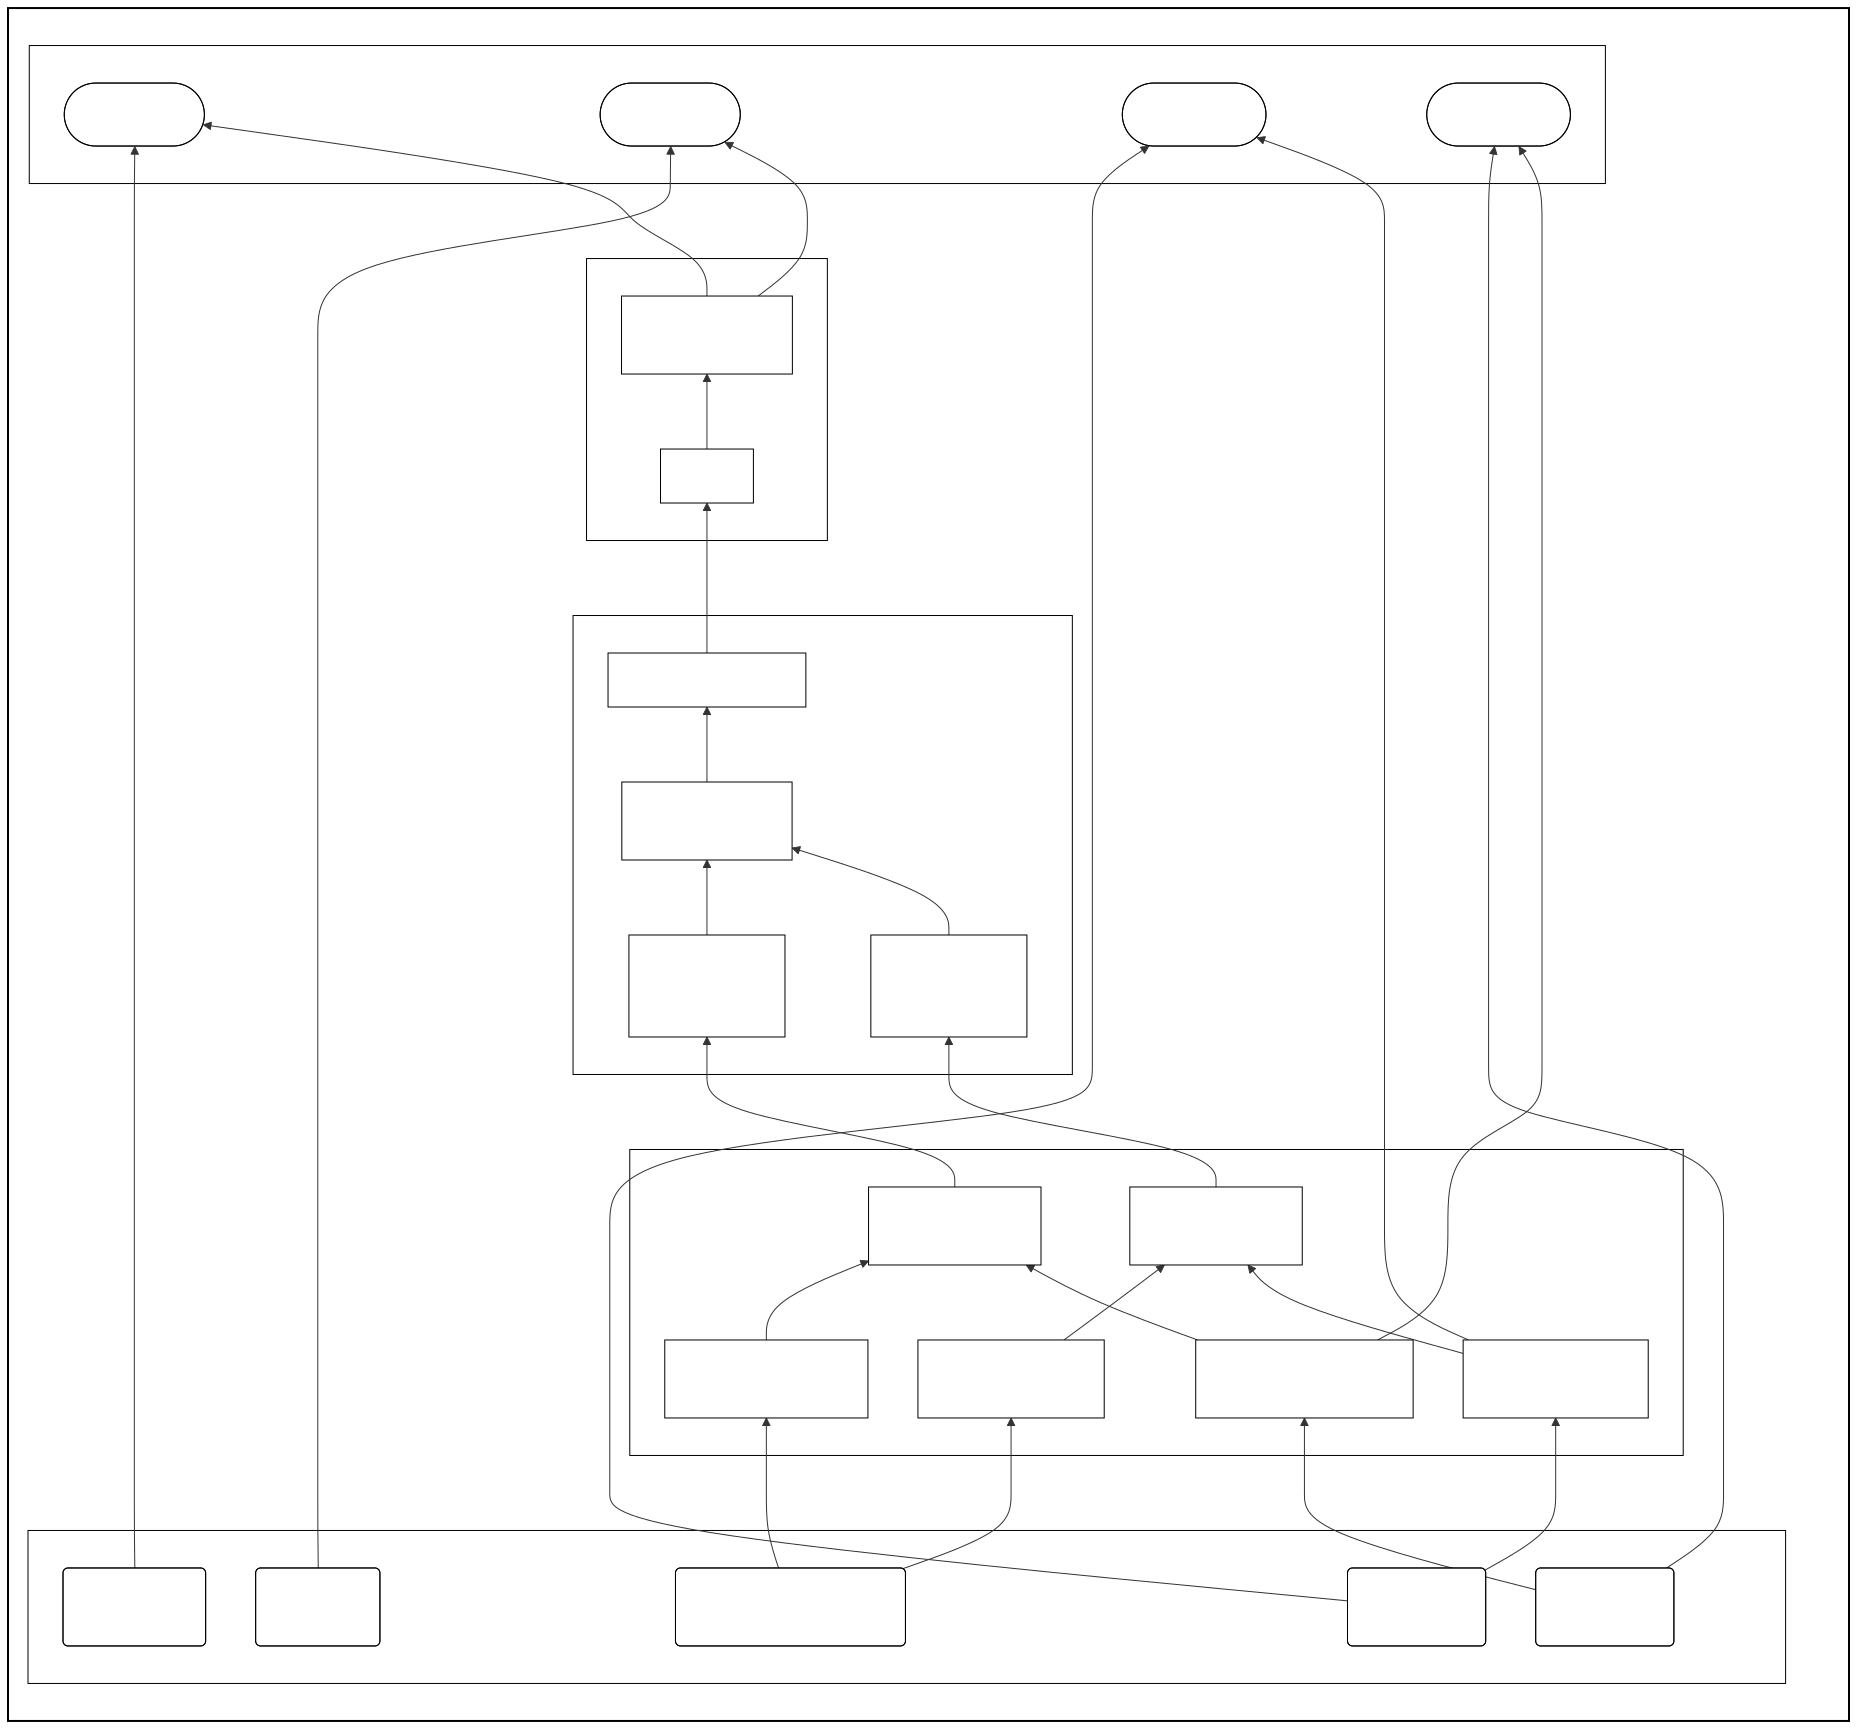
\includegraphics[width=1.0\textwidth]{img/idkt_arch.png}
    \caption{The iDKT Architecture. The diagram illustrates the five functional stages: (1) Input Data ingestion including BKT targets, (2) Individualized Embeddings, (3) the Transformer Core, (4) the MLP-based Output, and (5) the Loss Functions for representational grounding.\label{idkt_arch}}
\end{figure}


\section{Embeddings} \label{sec_embeddings}

In standard educational datasets, such as ASSISTments 2009, ASSISTments 2015, Algebra 2005, and others \citep{liu2022pykt}, student interactions are recorded at the level of specific questions or tasks, each of which is associated with one or more underlying concepts or knowledge components. This structure reflects the fact that proficiency in a concept (e.g., the Pythagorean Theorem) is acquired through interactions with a diverse range of tasks. While all tasks involving a concept share the same semantic core, they differ in their specific manifestations—most notably in their intrinsic difficulty or complexity. Therefore, an effective representation must capture both the shared identity of the concept and the unique deviation of the specific task.

In Transformer-based models \citep{vaswani2017attention} we can operationalize this principle representing the tasks as embedding vectors: 

\begin{equation}
    x' = c + u \cdot d \quad \text{(Task)}
\end{equation}


In this formulation, $c$ acts as the \textit{Concept Anchor}, a vector representing the invariant semantic identity of the concept while the vector $d$ represents the learnable \textit{Question Variation Axis}, defining the specific direction of the "transition gap". The scalar $u$ serves as the \textit{Relational Magnitude}, representing the question's specific relative difficulty compared to other questions involving the same concept. Consequently, rather than encode arbitrary embeddings for every question, we encode the vector sum of two distinct components with clear semantic meaning: a base \textit{concept identity} and a \textit{difficulty shift}. 

In a similar way, we can operationalize the interactions between questions and students as embedding vectors: 

\begin{equation}
    y' = e + u \cdot (f + d) \quad \text{(Interaction History)}
\end{equation}

Here $e$ represents the \textit{Interaction Base}, which is a combined representation of concept c and the binary outcome r (correct/incorrect), while $f$ represents the \textit{Interaction Variation Axis}, which is similar to the Question Variation Axis ($d_c$) but is specific to the interaction between a question and a student. The inclusion of $d_c$ in the interaction shift ensures that the difficulty vectors are consistent across both questions ($x'$) and interactions ($y'$).

Extending this rationale, we can enrich the $x'$ embeddings by integrating additional components with explicit semantic significance. Specifically, by adopting Bayesian Knowledge Tracing (BKT) as a reference model, we can incorporate vectors corresponding to its core theoretical parameters—Initial Knowledge ($L_0$) and Learning Rate ($T$)—thereby grounding the deep representation in established pedagogical constructs. 

To get individualized values for these parameters, we decompose them into population-level bases and student-specific deviations: 

\begin{equation} \label{eq_lc}
    l_c = L_{0} + k_s \cdot d_{k} \quad \text{(Personalized Initial Knowledge)}
\end{equation}
\begin{equation} \label{eq_tc}
    t_c = T + v_s \cdot d_{v} \quad \text{(Personalized Learning Rate)}
\end{equation}


where $l_c$ is the personalized initial knowledge for concept, $t_c$ is the personalized learning rate for concept, $L_{0}$ and $T$ are the population-level base embeddings, $d_{k}$ and $d_{v}$ are the learnable variation axes vectors (similar to the difficulty axis $d$), and $k_s$ and $v_s$ are the scalar student-specific deviations learned for each individual.

We include these vectors to get the final input embedding for the encoder and decoder components of the Transformer: 
\begin{equation}
    x' = (c + u \cdot d) - l_c \quad \text{(Individualized Task)}
\end{equation}
\begin{equation}
    y' = (e + u \cdot (f + d)) + t_c \quad \text{(Individualized Interaction History)}
\end{equation}

where $c$ represents the concept embedding, $u$ the question-specific difficulty shift, $d$ the task variation axis, $e$ the interaction base, $f$ the interaction variation axis, $l_c$ the personalized initial knowledge, and $t_c$ the personalized learning rate.

The rationale for using difference for the individualized task ($x'$) and sum for the interaction history ($y'$) is due to their distinct semantic roles:
\begin{itemize}
    \item $x'$ represents the $\textit{Transition Gap}$: $\textit {Difficulty} - \textit{Proficiency}$. Under this relational logic, objective task difficulty is offset by prior proficiency, ensuring that task demands are defined relative to the subject's baseline. This formulation captures the difference between the task requirements and the current state, representing the residual gap after accounting for latent proficiency.
    \item $y'$ represents the $\textit{Transition Gain}$: $\textit{Interaction} + \textit{Rate}$. The history encoder accumulates evidence from interactions, applying a consistent relational logic where the signal value is augmented by latent rate, ensuring that interaction outcomes are defined relative to the subject's pace. Under this formulation, the total value encompasses not only the interaction outcome but also the rate of progress through the state trajectory, as this incremental gain serves as a robust indicator of future performance. This approach, therefore, captures latent progression by augmenting observed outcomes with transition rate, thereby reflecting individualized acquisition rates.
\end{itemize}

\section{Loss Functions} \label{sec_loss}

The model is trained using a multi-objective loss function designed to ensure that the high-capacity Transformer remains aligned with pedagogical principles through Representational Grounding. The total loss $\mathcal{L}_{total}$ is defined as a weighted sum of different loss components described in detail below. 
\begin{equation}
    \mathcal{L}_{total} = L_{sup} + \lambda_{ref} L_{ref} + \lambda_{init} L_{init} + \lambda_{rate} L_{rate} + L_{reg}
\end{equation}

\subsection{Supervised Alignment ($L_{sup}$)}
The primary objective $L_{sup}$ uses standard Binary Cross-Entropy (BCE) between the iDKT performance predictions $\hat{y}_t$ and the observed ground truth outcomes $r_t \in \{0, 1\}$. This loss ensures predictive accuracy by minimizing the deviance from observed student behavior:
\begin{equation}
    L_{sup} = -\frac{1}{N} \sum_{t=1}^N [r_t \log(\hat{y}_t) + (1-r_t) \log(1-\hat{y}_t)]
\end{equation}

\subsection{Representational Grounding}
The grounding losses ($L_{ref}, L_{init}, L_{rate}$) use Mean Squared Error (MSE) to anchor deep representations to BKT-derived values. Specifically, $L_{ref}$ forces behavioral predictions to stay close to the theoretical baseline, while $L_{init}$ and $L_{rate}$ ground the individualized parameters $l_c$ and $t_c$ in meaningful educational starting points and acquisition paces, respectively. Instead of arbitrary latent weights, the model's internal states are projected through a sigmoid activation $\sigma(\cdot)$ and compared directly to the reference values:
\begin{align}
    L_{ref} &= \text{MSE}(\hat{y}, p_{BKT}) \\
    L_{init} &= \text{MSE}(\sigma(\bar{l}_c), L0_{BKT}) \\
    L_{rate} &= \text{MSE}(\sigma(\bar{t}_c), T_{BKT})
\end{align}
where $\bar{l}_c$ and $\bar{t}_c$ are the average across the feature dimension of the individualized embeddings for proficiency and rate, respectively. This formulation forces the deep representation to be not only predictive but also semantically consistent with the reference constructs.

\subsection{Inductive Bias Regularization ($L_{reg}$)}
While the grounding losses anchor the global position of the latent space to the BKT parameter estimations, $L_{reg}$ ensures that student-level individualization is \textit{parsimonious}. This loss acts directly on the individualization parameters ($u_q, k_s, v_s$) to ensure that the model only deviates from the theoretical prior when functionally necessary. We apply distinct $L_2$ penalties to the scalar parameters governing variation:
\begin{equation}
    L_{reg} = \lambda_{\text{u}} \sum_{q \in Q} u_q^2 + \lambda_{\text{k}} \sum_{s \in S} k_s^2 + \lambda_{\text{v}} \sum_{s \in S} v_s^2
\end{equation}
where $u_q$ represents item difficulty, $k_s$ is the student-specific knowledge gap, and $v_s$ is the learning rate deviation. This formulation implements a \textit{normal student prior}: the model assumes every subject adheres to the population-level parameters derived from the BKT reference unless their unique interaction history provides sufficient signal to justify the regularization cost. 

\section{Results and Discussion} \label{sec_experiment}

\subsection{Research Questions}

The experimental validation of iDKT is guided by the following research questions:

\begin{enumerate}
    \item \textbf{Interpretability Validation (RQ1)}: Is it possible to rigorously validate that a iDKT model, whose representations are grounded in a reference model, actually yields interpretable constructs?
    \item \textbf{Trade-Off between Predictive Performance and Interpretability (RQ2)}: To what extent can deep knowledge tracing models be constrained for interpretability alignment without significantly degrading predictive performance?
    \item \textbf{Improvement of Pedagogical Diagnostics (RQ3)}: How can the Transformer’s ability to capture longitudinal context be utilized to improve or complement pedagogical diagnostics?
\end{enumerate}

\subsection{Experimental Setup}

We implemented the iDKT model in \texttt{PyTorch} and used the benchmark library \texttt{PYKT} \citep{liu2022pykt} to leverage standardized data preprocessing, dataset splitting and benchmarking of baseline models. For training, we used standard 5-fold cross-validation with an 80/20 train/test split. The model was trained using the Adam optimizer with a learning rate of $1e-4$, a batch size of 64, and a dropout rate of 0.2 to prevent overfitting. The maximum number of epochs was set to 200, with an early stopping mechanism (patience=10) to terminate training if validation performance plateaued.

The Transformer architecture was configured with an embedding dimension $d_{model}$ of 256, 8 attention heads, and 4 encoder/decoder blocks. The feed-forward dimension $d_{ff}$ was set to 512. Regularization penalties for individualization parameters ($L_2$ on $u_q$, $k_s$, $v_s$) were all set to $1e-5$. For reproducibility, all experiments were seeded (seed=42) and executed on NVIDIA A100 GPU infrastructure. Predictive performance was evaluated using Area Under the ROC Curve (AUC) and Accuracy (ACC), while interpretability was assessed using the metrics defined in Section \ref{sec_validation}.

\subsection{Datasets}\label{sec_dataset}

We did the evaluation of iDKT with these 5 widely used datasets: 

• ASSISTments2009: A dataset consisting of math exercises, collected from the free online
tutoring ASSISTments platform in 2009-2010. It is one of the most widely used and has been the standard benchmark for many years \citep{feng2009addressing}.

• ASSISTments2015: This dataset was collected from the ASSISTments platform in the year of 2015. It has the largest number of students among the other ASSISTments datasets \citep{feng2009addressing}.

• Algebra2005: A dataset from the KDD Cup 2010 EDM Challenge containing questions from the Carnegie Learning Algebra system deployed 2005-2006 \citep{stamper2010algebra}.

• Bridge2006: A dataset from the KDD Cup 2010 EDM Challenge with the Carnegie Learning Bridge to Algebra system, deployed 2006-2007 \citep{stamper2010bridge}.

• NIPS34: A dataset collected from the Eedi platform \citep{wang2020instructions} containing answers to multiple-choice diagnostic math questions for the Tasks 3 \& 4 at the NeurIPS 2020 Education Challenge. 


\subsection{Predictive Performance}

To evaluate the predictive performance of the iDKT model, we used the Area Under the Curve (AUC) and the Classification Accuracy (ACC) of the models on the test set with the 5 datasets described in Section \ref{sec_dataset}. The results are shown in the Table \ref{tab_performance}.


\begin{table}[htbp] 
%\small % Change table font size
\caption{Predictive Performance of the iDKT model across 5 datasets.\label{tab_performance}}
%\isPreprints{\centering}{} % Only used for preprints
\begin{tabularx}{\textwidth}{lccccc}
\toprule
\textbf{Model} & \textbf{AS2009\_S} & \textbf{AS2015} & \textbf{Algebra2005} & \textbf{Bridge2006} & \textbf{NIPS34} \\
\midrule
iDKT & 0.8255 & 0.7252 & 0.9281 & 0.8092 & 0.7987 \\
\bottomrule
\end{tabularx}
\end{table}

When comparing these results with state-of-the-art DKT models reported in \citep{liu2022pykt}, we observe that iDKT achieves the best predictive performance on the AS2009 and Algebra2005 datasets and ranks second on the Bridge2006 and NIPS34 datasets, surpassed only by the AKT model.

\subsection{Interpretability Validation (RQ1)} \label{sec_validation}


To verify that iDKT’s internal representations—specifically Personalized Initial Knowledge ($\mathbf{l}_c$) and Personalized Learning Rate ($\mathbf{t}_c$) as defined in Equations \ref{eq_lc} and \ref{eq_tc}—faithfully represent the educational constructs postulated by the reference model, we employ two metrics widely utilized in psychometrics and educational measurement \citep{campbell1959convergent, american1985standards}: 

\begin{enumerate}
    \item \textit{Convergent Validity (Latent Fidelity)}: This metric, denoted as $I_1$, is calculated as the Pearson correlation ($r$) between the projected latent factors ($l_u, t_u$) and the reference BKT parameters ($L_{0}$ and $T$). High alignment proves the model has successfully internalized the theoretical constructs. 
    
    The metrics are expressed as:
    \begin{equation} \label{eq_i1}
    I_{1l} = \text{Corr}(l_u, L_{0}) \quad \text{and} \quad I_{1t} = \text{Corr}(t_u, T)
    \end{equation}
    where the projected latent factors are calculated via:
    \begin{equation} \label{eq_projection}
    l_u = \sigma(\bar{l}_c), \quad t_u = \sigma(\bar{t}_c)
    \end{equation}
    with $\bar{l}_c$ and $\bar{t}_c$ representing the mean across the feature dimension of the individualized embeddings.
    \item \textit{Predictor Equivalence (Behavioral Alignment)}: This metric, denoted as $I_2$, assesses the functional substitutability of iDKT parameters by executing a \textit{cross-model simulation}. We "inject" the projected iDKT parameters ($l_u$ and $t_u$) into the canonical BKT recurrence equations to generate \textit{induced mastery trajectories}. This allows us to verify whether the learned factors preserve their causal roles. The metric is statistically quantified as the Pearson correlation coefficient between these induced trajectories and the theoretical reference trajectories generated by the original BKT model:
    \begin{equation} \label{eq_i2}
    I_2 = \text{Corr}\left( P(L)_{ind}, P(L)_{ref} \right)
    \end{equation}
    where $P(L)_{ind}$ and $P(L)_{ref}$ represent the sequences of mastery probabilities at each timestep for the induced and reference models, respectively.
\end{enumerate}

Table \ref{tab_interpretability} shows interpretability metrics for the unconstrained iDKT model ($\lambda_{ref}=0$).

\begin{table}[htbp]
\caption{Interpretability Alignment Metrics for unconstrained iDKT ($\lambda_{ref}=0$). \label{tab_interpretability}}
\footnotesize
\begin{tabularx}{\textwidth}{lcccccc}
\toprule
\textbf{Dataset} & \textbf{$I_1$ (Init.)} & \textbf{Int.} & \textbf{$I_1$ (Rate)} & \textbf{Int.} & \textbf{$I_2$} & \textbf{Int.} \\
\midrule
AS2009 & -0.1382 & Poor & -0.0067 & Negl. & 0.1870 & Poor \\
AS2015 & -0.0392 & Negl. & 0.0908 & Negl. & 0.0975 & Negl. \\
Algebra2005 & -0.0602 & Negl. & -0.0273 & Negl. & 0.0600 & Negl. \\
Bridge2006 & -0.0645 & Negl. & 0.0160 & Negl. & 0.0809 & Negl. \\
NIPS34 & 0.2070 & Poor & -0.0425 & Negl. & 0.1722 & Poor \\
\bottomrule
\end{tabularx}
\end{table}

Upon enabling Representational Grounding ($\lambda_{ref}=0.10$), we observe a significant restoration of semantic alignment, as detailed in Table \ref{tab_interpretability_grounded}.

\begin{table}[htbp]
\caption{Interpretability Alignment Metrics for grounded iDKT ($\lambda_{ref}=0.1$). \label{tab_interpretability_grounded}}
\footnotesize
\begin{tabularx}{\textwidth}{lcccccc}
\toprule
\textbf{Dataset} & \textbf{$I_1$ (Init.)} & \textbf{Int.} & \textbf{$I_1$ (Rate)} & \textbf{Int.} & \textbf{$I_2$} & \textbf{Int.} \\
\midrule
AS2009\_S & 0.5409 & Good & 0.3131 & Fair & 0.6250 & Excell. \\
AS2015 & 0.9217 & Excell. & 0.8801 & Excell. & 0.1749 & Poor \\
Algebra2005 & 0.5444 & Good & 0.3310 & Fair & 0.0661 & Negl. \\
Bridge2006 & 0.4561 & Fair & 0.6422 & Good & 0.0859 & Negl. \\
\bottomrule
\end{tabularx}
\end{table}


The results presented in Tables \ref{tab_interpretability} and \ref{tab_interpretability_grounded} reveal a notable divergence between \textit{Convergent Validity} ($I_1$) and \textit{Predictor Equivalence} ($I_2$). Although $I_1$ attains high levels across most datasets even with relatively low $\lambda_{ref}$ grounding weights, $I_2$ remains consistently low.

High $I_1$ scores demonstrate that iDKT successfully internalizes the \textit{semantic identity} of the theoretical constructs (Initial Knowledge and Learning Rate). However, $I_2$ measures functional substitutability within a comparatively constrained reference model that is unable to capture the intricate behavioral patterns identified by iDKT. As a high-capacity Transformer, iDKT captures complex, long-range dependencies and context-aware dynamics that exceed the modeling capability of classical BKT. This discrepancy provides empirical evidence that iDKT does not merely mimic the reference model, but rather maps its core pedagogical constructs onto a more sophisticated and predictive architecture.


\subsection{Accuracy--Interpretability Trade-Off (RQ2)} \label{sec_tradeoff}

Prediction performance and interpretability are considered as two opposing goals. Our approach to explore such trade-off is based in building a Pareto frontier, which is constructed by gradually increasing the grounding weight $\lambda_{ref}$ defined in Equation \ref{eq_loss} and plotting the resulting values of performance and interpretability. 

We measure interpretability using the \textit{Composite Alignment} $\bar{I}$ metric, defined as the arithmetic mean of the individual alignment components $I_1$ and $I_2$ defined in Equations \ref{eq_i1} and \ref{eq_i2}:

\begin{equation} \label{eq_composite_i}
I = \frac{1}{3} \left( I_{1l} + I_{1t} + I_{2} \right)
\end{equation}

Tables \ref{tab_pareto_as2015} and \ref{tab_pareto_as2009} summarize the performance and alignment results for the ASSISTments 2009 and 2015 datasets across a systematic sweep of the grounding weight $\lambda_{ref}$ (Equation \ref{eq_loss}). 

Figures \ref{fig_pareto_as2015} and \ref{fig_pareto_as2009} illustrate the resulting Pareto frontiers. We observe that theoretical guidance serves as a powerful regularizer, although the \textit{Saturation Point} (the weight at which interpretability is maximized) varies by dataset complexity. For the problem-level \textit{ASSISTments 2009}, synergy is achieved at $\lambda=0.10$ and saturation at $\lambda=0.30$. Conversely, the concept-level \textit{ASSISTments 2015} reaches saturation faster at $\lambda=0.10$, retaining 99.9\% of accuracy. Beyond these points, we observe a \textit{grounding collapse} in both datasets, where the model fails to reconcile excessive constraints with behavioral evidence.

\begin{figure}[htbp]
\centering
\captionof{table}{Pareto Sweep results for ASSISTments 2015. \label{tab_pareto_as2015}}
\footnotesize
\begin{tabularx}{\textwidth}{lccc}
\toprule
\textbf{$\lambda_{ref}$} & \textbf{Performance (AUC)} & \textbf{Interpretability (I)} & \textbf{Interpretation} \\
\midrule
0.0 (Baseline) & 0.7248 & -0.0012 & Black Box \\
0.1 (Saturation Point) & 0.7245 & 0.6673 & 99.9\% AUC Retained \\
0.2 & 0.7181 & 0.6453 & High-Fidelity Diagnostic \\
0.3 & 0.7112 & 0.6095 & Latent Degradation \\
0.4 & 0.7047 & 0.6377 & Latent Degradation \\
0.5 & 0.6975 & 0.5691 & Theory-Dominant \\
0.6 & 0.6918 & 0.5337 & Latent Degradation \\
0.7 & 0.6874 & 0.5331 & Latent Degradation \\
0.8 & 0.6830 & 0.4828 & Grounding Collapse \\
1.0 & 0.6763 & 0.4828 & Grounding Collapse \\
\bottomrule
\end{tabularx}

\vspace{10em}

\includegraphics[width=1.0\textwidth]{img/pareto_as2015.png}
\caption{iDKT Pareto Frontier for ASSISTments 2015. The trajectory illustrates a saturation of theoretical alignment at $\lambda \approx 0.2$, followed by a drift at higher weights where performance is traded without gaining interpretability. \label{fig_pareto_as2015}}
\end{figure}


\begin{figure}[htbp]
\centering
\captionof{table}{Pareto Sweep results for ASSISTments 2009. \label{tab_pareto_as2009}}
\footnotesize
\begin{tabularx}{\textwidth}{lccc}
\toprule
\textbf{$\lambda_{ref}$} & \textbf{Performance (AUC)} & \textbf{Interpretability (I)} & \textbf{Interpretation} \\
\midrule
0.0 (Baseline) & 0.8207 & 0.0293 & Unconstrained Black Box \\
0.1 (Synergy Spot) & 0.8255 & 0.3846 & Accuracy-Interpretability Synergy \\
0.2 & 0.8110 & 0.4270 & Theory-Balanced Inductive Bias \\
0.3 (Saturation Point) & 0.7963 & 0.4790 & Theoretical Saturation (Max Int.) \\
0.4 & 0.7824 & 0.2740 & Non-monotonicity \\
0.5 & 0.7760 & 0.4125 & Grounding Degradation \\
0.6 & 0.7692 & 0.3587 & Grounding Degradation \\
0.7 & 0.7629 & 0.2781 & Grounding Degradation \\
0.8 & 0.7552 & 0.0708 & Grounding Collapse \\
1.0 & 0.7501 & 0.0714 & Grounding Collapse \\
\bottomrule
\end{tabularx}

\vspace{10em}

\includegraphics[width=1.0\textwidth]{img/pareto_as2009.png}
\caption{iDKT Pareto Frontier for ASSISTments 2009. The curve displays a \textit{synergy point} where performance peaks at $\lambda = 0.1$, followed by a \textit{grounding collapse} as excessive constraints over-regularize the latent space. \label{fig_pareto_as2009}}
\end{figure}

\subsection{Improvement of Pedagogical Diagnostics (RQ3)} \label{sec_gran_results}

In the following sections, we analyze how the architectural design of iDKT can be leveraged to improve pedagogical diagnostics 

\subsubsection{Contextualization} \label{sec_longitudinal}

The capability of iDKT to leverage longitudinal context is illustrated in Figure \ref{fig_mastery_866}, which contrasts its mastery estimations with the BKT baseline for a high-proficiency learner. While BKT leads to excessive volatility---where isolated failures are interpreted as significant knowledge drops---iDKT maintains a stable and resilient diagnostic trajectory. 

The core of this advantage lies in the self-attention mechanism, which enables iDKT to encode longitudinal context by dynamically weighting the entire interaction history. Instead of relying solely on the most recent state, iDKT evaluates each interaction in the context of the student's established behavioral patterns. In the scenario shown in Figure \ref{fig_mastery_866}, the model maintains a high mastery estimation despite sporadic failures because the attention weights remain anchored to the student's longitudinal progression. This capacity to distinguish between temporary behavioral noise (e.g., slips) and genuine changes in knowledge state represents a fundamental improvement over classical baselines, supporting robust and individualized diagnostics.

\begin{figure}[htbp]
\centering
\includegraphics[width=0.75\textwidth]{img/idkt_mastery_866.png}
\caption{Comparison of two mastery trajectories estimated by iDKT and BKT illustrating how iDKT can be more stable and resilient against behavioral noise. \label{fig_mastery_866}} 
\end{figure} 


\subsubsection{Individualization} 

The primary value of iDKT lies in its ability to transform population-level theoretical averages into high-granular contextual diagnostics. While standard BKT assumes that every student shares a fixed initial mastery ($L_0$) and learning rate ($T$) for a given skill, iDKT decomposes these into individualized profiles.

To statistically quantify this granularity, we analyze the \textit{delta distribution} ($\Delta = t_s - T$), representing the student-specific deviation from the theoretical learning rate across all skills. In both ASSISTments datasets, we observe a significant non-zero standard deviation ($\sigma \approx 0.019$ for AS2009 and $\sigma \approx 0.039$ for AS2015). This represents a substantial increase in diagnostic resolution compared to the BKT baseline, where $\sigma = 0$. The right-skewed tail in the distributions identifies a sub-population of fast learners whose true acquisition pace is systematically underestimated by classical models.

Figure \ref{fig_delta} visualizes the delta distributions for both datasets. The width of the curves quantifies the pedagogical information that is lost when using population-level averages. This variance allows the system to distinguish between students who are faster than suggested by theoretical priors and those who require additional practice to reach mastery.

\subsubsection{High-Granularity Trajectory Analysis} \label{sec_mosaic_analysis}

To provide definitive visual evidence for RQ3, we generated a Mastery Alignment Mosaic (Figure~\ref{fig_mosaic}) displaying individualized trajectories for three learning archetypes (Fast, Median, Slow) across 15 skills. For rigorous validation, we utilized the ``Set S Isolation'' strategy, restricting the analysis to students with continuous interaction histories ($\le 200$ steps) and recalibrating the BKT reference exclusively on this population.

\begin{figure}[htbp]
\centering
\includegraphics[width=1.0\textwidth]{img/mastery_alignment_mosaic_real.png}
\caption{Mastery Trajectory Alignment Mosaic for AS2009\_S. Solid lines represent iDKT individualized mastery, while dashed lines show the BKT baseline. Markers indicate observed student performance (Circle: Correct, X: Incorrect). Trajectories are selected from students with $>10$ interactions per skill. \label{fig_mosaic}}
\end{figure}

The qualitative analysis of these trajectories reveals three significant pedagogical insights:
\begin{enumerate}
    \item \textbf{Dynamic Diagnostic Placement}: Even when BKT is forced to start at the population prior ($L_0$), iDKT starting points ($t=1$) vary per student. This demonstrates that iDKT leverages cross-skill behavioral transfers to perform individualized placement before the first interaction with a new skill.
    \item \textbf{Trajectory Crossovers}: We observe instances where students starting with lower initial mastery overtake peers due to a higher identified learning velocity ($t_s$). This confirms iDKT's ability to model individualized acquisition rates beyond population-level curves.
    \item \textbf{Diagnostic Resilience}: iDKT displays superior stability compared to BKT baselines. While isolated failures cause sharp drops in BKT dashed lines, iDKT solid lines for high-velocity learners remain stable, correctly identifying temporary slips vs.\ fundamental knowledge loss.
\end{enumerate}

\subsubsection{Confidence} \label{sec_confidence}

Individualized student profiling offers new opportunities for pedagogical monitoring and adaptive intervention. A significant practical application is evaluating the reliability of predictions made by intrinsically interpretable models, such as BKT. By comparing BKT mastery estimations with those from iDKT, we can derive a measure of pedagogical confidence in the theoretical baseline. 

This relationship is visualized in Figure \ref{fig_heatmaps}, which displays the concordance between BKT and iDKT mastery predictions across the sub-population of the most frequent skills and students for both datasets. The ASSISTments 2015 results demonstrate high levels of agreement, whereas the ASSISTments 2009 data reveals more divergence, where iDKT uncovers individualized patterns beyond the theoretical prior. Such visualizations provide actionable pedagogical insights that complement traditional baseline diagnostics. 
This visualization framework provides robust support for personalized longitudinal tracking by identifying students or curricular content that deviate from theoretical expectations. These divergences serve as critical diagnostic indicators for cases that may warrant prioritized pedagogical intervention.

\begin{figure}[htbp]
    \centering
    \includegraphics[width=\textwidth]{img/per_skill_alignment_predictions_2015.png}\\
    {\small (a) ASSISTments 2015}\\[10pt]
    \includegraphics[width=\textwidth]{img/per_skill_alignment_predictions_2009.png}\\
    {\small (b) ASSISTments 2009}
    \caption{Heatmaps of per-skill prediction alignment. \label{fig_heatmaps}}
\end{figure}




%%%%%%%%%%%%%%%%%%%%%%%%%%%%%%%%%%%%%%%%%%
\section{Conclusions}\label{sec_conclusions}

This work has introduced iDKT, a Transformer-based Knowledge Tracing model that bridges the gap between the high predictive capacity of deep learning and the intrinsic interpretability of models such as BKT, which utilize constructs with clear semantic meanings. By utilizing Representational Grounding, we have demonstrated that it is possible to anchor deep latent representations to semantically meaningful constructs without sacrificing state-of-the-art performance.

Our experimental results successfully address the research questions. First, we proved that iDKT successfully internalizes the theoretical constructs of the reference model, achieving high convergent validity ($I_1$). Second, we formalized a methodology for measuring the trade-off between predictive performance and interpretability, enabling the identification of the ``Interpretability Sweet Spot'' where significant alignment is achieved with minimal loss in predictive AUC. Finally, we demonstrated that iDKT provides a high increase in diagnostic granularity compared to population-level baselines by identifying individualized learning velocities that enable truly adaptive pacing.

The primary contribution of this research is twofold: a robust methodology for evaluating the internal interpretability of Transformer-based models in education, and a practical architecture that transforms ``black-box'' predictors into interpretable tools for knowledge tracing. By grounding deep learning in established educational concepts, iDKT offers a path toward AI-driven personalization that is both highly accurate and pedagogically actionable, providing a foundation for next-generation intelligent tutoring systems.


%%%%%%%%%%%%%%%%%%%%%%%%%%%%%%%%%%%%%%%%%%
\vspace{6pt} 

%%%%%%%%%%%%%%%%%%%%%%%%%%%%%%%%%%%%%%%%%%
%% optional
%\supplementary{The following supporting information can be downloaded at:  \linksupplementary{s1}, Figure S1: title; Table S1: title; Video S1: title.}

% Only for journal Methods and Protocols:
% If you wish to submit a video article, please do so with any other supplementary material.
% \supplementary{The following supporting information can be downloaded at: \linksupplementary{s1}, Figure S1: title; Table S1: title; Video S1: title. A supporting video article is available at doi: link.}

% Only used for preprtints:
% \supplementary{The following supporting information can be downloaded at the website of this paper posted on \href{https://www.preprints.org/}{Preprints.org}.}

% Only for journal Hardware:
% If you wish to submit a video article, please do so with any other supplementary material.
% \supplementary{The following supporting information can be downloaded at: \linksupplementary{s1}, Figure S1: title; Table S1: title; Video S1: title.\vspace{6pt}\\
%\begin{tabularx}{\textwidth}{lll}
%\toprule
%\textbf{Name} & \textbf{Type} & \textbf{Description} \\
%\midrule
%S1 & Python script (.py) & Script of python source code used in XX \\
%S2 & Text (.txt) & Script of modelling code used to make Figure X \\
%S3 & Text (.txt) & Raw data from experiment X \\
%S4 & Video (.mp4) & Video demonstrating the hardware in use \\
%... & ... & ... \\
%\bottomrule
%\end{tabularx}
%}

%%%%%%%%%%%%%%%%%%%%%%%%%%%%%%%%%%%%%%%%%%
\authorcontributions{Conceptualization, C. L.; methodology, C. L. and O. C. S.; software, C. L.; validation, C. L. and O. C. S.; formal analysis, C. L.; investigation, C. L.; resources, C. L. and O. C. S.; data curation, C. L.; writing---original draft preparation, C. L.; writing---review and editing, C. L. and O. C. S.; visualization, C. L.; supervision, O. C. S.; project administration, O. C. S.; funding acquisition, O. C. S. All authors have read and agreed to the published version of the manuscript.}

\funding{This research received no external funding.}

\dataavailability{The datasets used in this paper can be downloaded through the links provided in https://pykt-toolkit.readthedocs.io/en/latest/datasets.html.}

\conflictsofinterest{The authors declare no conflicts of interest.} 

%%%%%%%%%%%%%%%%%%%%%%%%%%%%%%%%%%%%%%%%%%
\begin{adjustwidth}{-\extralength}{0cm}
%\printendnotes[custom] % Un-comment to print a list of endnotes

\reftitle{References}

% Please provide either the correct journal abbreviation (e.g. according to the “List of Title Word Abbreviations” http://www.issn.org/services/online-services/access-to-the-ltwa/) or the full name of the journal.
% Citations and References in Supplementary files are permitted provided that they also appear in the reference list here. 

%=====================================
% References, variant A: external bibliography
%=====================================
\bibliography{biblio}

%=====================================
% References, variant B: internal bibliography (commented out)
%=====================================

% ACS format
% \isAPAandChicago{}{%
% \begin{thebibliography}{999}
% % Reference 1
% \bibitem[Author1(year)]{ref-journal}
% Author~1, T. The title of the cited article. {\em Journal Abbreviation} {\bf 2008}, {\em 10}, 142--149.
% ... (truncated for chunk)

% % Chicago format (Used for journal: arts, genealogy, histories, humanities, jintelligence, laws, literature, religions, risks, socsci)
% \isChicagoStyle{%
% \begin{thebibliography}{999}
% % Reference 1
% \bibitem[Aranceta-Bartrina(1999a)]{ref-journal}
% Aranceta-Bartrina, Javier. 1999a. Title of the cited article. \textit{Journal Title} 6: 100--10.
% % Reference 2
% \bibitem[Aranceta-Bartrina(1999b)]{ref-book1}
% Aranceta-Bartrina, Javier. 1999b. Title of the chapter. In \textit{Book Title}, 2nd ed. Edited by Editor 1 and Editor 2. Publication place: Publisher, vol. 3, pp. 54–96.
% % Reference 3
% \bibitem[Baranwal and Munteanu {[1921]}(1955)]{ref-book2}
% Baranwal, Ajay K., and Costea Munteanu. 1955. \textit{Book Title}. Publication place: Publisher, pp. 154--96. First published 1921 (op-tional).
% % Reference 4
% \bibitem[Berry and Smith(1999)]{ref-thesis}
% Berry, Evan, and Amy M. Smith. 1999. Title of Thesis. Level of Thesis, Degree-Granting University, City, Country. Identifi-cation information (if available).
% % Reference 5
% \bibitem[Cojocaru et al.(1999)]{ref-unpublish}
% Cojocaru, Ludmila, Dragos Constatin Sanda, and Eun Kyeong Yun. 1999. Title of Unpublished Work. \textit{Journal Title}, phrase indicating stage of publication.
% % Reference 6
% \bibitem[Driver et al.(2000)]{ref-proceeding}
% Driver, John P., Steffen Rohrs, and Sean Meighoo. 2000. Title of Presentation. In \textit{Title of the Collected Work} (if available). Paper presented at Name of the Conference, Location of Conference, Date of Conference.
% % Reference 7
% \bibitem[Harwood(2008)]{ref-url}
% Harwood, John. 2008. Title of the cited article. Available online: URL (accessed on Day Month Year).
% \end{thebibliography}
% }{}
% 
% % APA format (Used for journal: admsci, behavsci, businesses, econometrics, economies, education, ejihpe, games, humans, ijfs, journalmedia, jrfm, languages, psycholint, publications, tourismhosp, youth)
% \isAPAStyle{%
% \begin{thebibliography}{999}
% % Reference 1
% \bibitem[\protect\citeauthoryear{Azikiwe \BBA\ Bello}{{2020a}}]{ref-journal}
% Azikiwe, H., \& Bello, A. (2020a). Title of the cited article. \textit{Journal Title}, \textit{Volume}(Issue), 
% Firstpage--Lastpage/Article Number.
% % Reference 2
% \bibitem[\protect\citeauthoryear{Azikiwe \BBA\ Bello}{{2020b}}]{ref-book1}
% Azikiwe, H., \& Bello, A. (2020b). \textit{Book title}. Publisher Name.
% % Reference 3
% \bibitem[Davison(1623/2019)]{ref-book2}
% Davison, T. E. (2019). Title of the book chapter. In A. A. Editor (Ed.), \textit{Title of the book: Subtitle} 
% (pp. Firstpage--Lastpage). Publisher Name. (Original work published 1623) (Optional).
% % Reference 4
% \bibitem[Fistek et al.(2017)]{ref-proceeding}
% Fistek, A., Jester, E., \& Sonnenberg, K. (2017, Month Day). Title of contribution [Type of contribution]. Conference Name, Conference City, Conference Country.
% % Reference 5
% \bibitem[Hutcheson(2012)]{ref-thesis}
% Hutcheson, V. H. (2012). \textit{Title of the thesis} [XX Thesis, Name of Institution Awarding the Degree].
% % Reference 6
% \bibitem[Lippincott \& Poindexter(2019)]{ref-unpublish}
% Lippincott, T., \& Poindexter, E. K. (2019). \textit{Title of the unpublished manuscript} [Unpublished manuscript/Manuscript in prepara-tion/Manuscript submitted for publication]. Department Name, Institution Name.
% % Reference 7
% \bibitem[Harwood(2008)]{ref-url}
% Harwood, J. (2008). \textit{Title of the cited article}. Available online: URL (accessed on Day Month Year).
% \end{thebibliography}
% }{}

% If authors have biography, please use the format below
%\section*{Short Biography of Authors}
%\bio
%{\raisebox{-0.35cm}{\includegraphics[width=3.5cm,height=5.3cm,clip,keepaspectratio]{Definitions/author1.pdf}}}
%{\textbf{Firstname Lastname} Biography of first author}
%
%\bio
%{\raisebox{-0.35cm}{\includegraphics[width=3.5cm,height=5.3cm,clip,keepaspectratio]{Definitions/author2.jpg}}}
%{\textbf{Firstname Lastname} Biography of second author}

% For the MDPI journals use author-date citation, please follow the formatting guidelines on http://www.mdpi.com/authors/references
% To cite two works by the same author: \citeauthor{ref-journal-1a} (\citeyear{ref-journal-1a}, \citeyear{ref-journal-1b}). This produces: Whittaker (1967, 1975)
% To cite two works by the same author with specific pages: \citeauthor{ref-journal-3a} (\citeyear{ref-journal-3a}, p. 328; \citeyear{ref-journal-3b}, p.475). This produces: Wong (1999, p. 328; 2000, p. 475)

%%%%%%%%%%%%%%%%%%%%%%%%%%%%%%%%%%%%%%%%%%
%% for journal Sci
%\reviewreports{\\
%Reviewer 1 comments and authors’ response\\
%Reviewer 2 comments and authors’ response\\
%Reviewer 3 comments and authors’ response
%}
%%%%%%%%%%%%%%%%%%%%%%%%%%%%%%%%%%%%%%%%%%
\PublishersNote{}
\end{adjustwidth}
\end{document}

